\documentclass[addpoints]{physlabs}

\labtitle{Geometrical Optics}
\labnum{}
\labnumroman{XII}
\course{PHYSICS 123 - 183}
\coursesubtitle{Waves and Modern Physics}
\date{\today}

\usetikzlibrary{patterns, patterns.meta, angles, calc, decorations.markings, decorations.pathreplacing, quotes, shapes, shapes.geometric, arrows.meta}

\begin{document}

\maketitle

% PRELAB SECTION
\begin{prelab}

    \filbreak
    \question[1] Draw the location of the image of an object placed near converging and diverging lenses, pictured below. Foci are indicated as black dots. Make sure you include at least two rays in each diagram, and answer whether the images are \textsl{real} or \textsl{virtual}, \textsl{erect} or \textsl{inverted}, and \textsl{reduced} or \textsl{magnified}.
    %
    \begin{figure*}[ht]
        \centering
        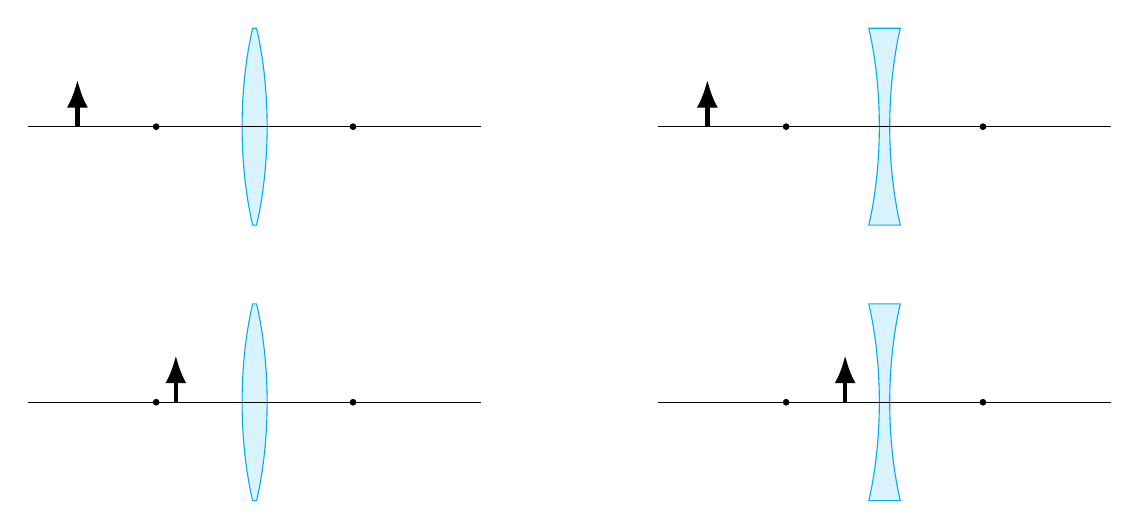
\begin{tikzpicture}
    \begin{scope}
        \def\L{4}           % near point
        \def\f{1.25}           % focal length
        \def\h{0.6}         % object height
        \def\p{1.8*\f}      % object-lens distance
        % Compute angles
        \def\tanalpha{\h / (\p - \f)}
        \def\tanbeta{\h / (\p)}
        % Draw the converging lens
        \draw[cyan, line join=round,fill=cyan!15] (0.025,-1.25) coordinate (L1) arc (-30:30:1 and 2.5) coordinate (L2) -- ++(-0.05,0) arc (150:210:1 and 2.5) -- cycle;
        % Draw the axial line and focal points
        \draw ({-2.3*\f}, 0) -- ({2.3*\f}, 0);
        \filldraw[black] (-\f, 0) circle (0.035);
        \filldraw[black] (\f, 0) circle (0.035);
        % Draw the object beyond the focal point
        \draw[ultra thick, -Latex] (-\p, 0) coordinate (O1) -- (-\p, \h) coordinate (O2);
        % Draw rays from the object to the image through the lens
       % \draw[red] (O2) -- (0,\h) -- (\f,0) -- ({(\f*\tanalpha)/(\tanbeta)}, {-\f*\tanalpha});
       % \draw[red] (O2) -- (-\f,0) -- (0,{-\f*\tanalpha}) -- ({(\f*\tanalpha)/(\tanbeta)}, {-\f*\tanalpha});
       % \draw[red] (O2) -- (0,0) -- ({(\f*\tanalpha)/(\tanbeta)}, {-\f*\tanalpha});
       % \draw[ultra thick, violet, -Latex] ({(\f*\tanalpha)/(\tanbeta)}, 0) -- ({(\f*\tanalpha)/(\tanbeta)}, {-\f*\tanalpha});
    \end{scope}
    %
    \begin{scope}[shift={(0,-3.5)}]
        \def\L{4}           % near point
        \def\f{1.25}           % focal length
        \def\h{0.6}         % object height
        \def\p{0.8*\f}      % object-lens distance
        % Draw the converging lens
        \draw[cyan, line join=round,fill=cyan!15] (0.025,-1.25) coordinate (L1) arc (-30:30:1 and 2.5) coordinate (L2) -- ++(-0.05,0) arc (150:210:1 and 2.5) -- cycle;
        % Draw the axial line and focal points
        \draw ({-2.3*\f}, 0) -- ({2.3*\f}, 0);
        \filldraw[black] (-\f, 0) circle (0.035);
        \filldraw[black] (\f, 0) circle (0.035);
        % Draw the object before the focal point
        \draw[ultra thick, -Latex] (-\p, 0) coordinate (O1) -- (-\p, \h) coordinate (O2);
    \end{scope}
    %
    \begin{scope}[shift={(8,0)}]
        \def\L{4}           % near point
        \def\f{1.25}           % focal length
        \def\h{0.6}         % object height
        \def\p{1.8*\f}      % object-lens distance
        % Draw the diverging lens
        \draw[cyan, line join=round, fill=cyan!15] (0.2,1.25) coordinate (L1) arc (150:210:1 and 2.5) -- ++(-0.4,0) coordinate (L2) arc (-30:30:1 and 2.5) -- cycle;
        % Draw the axial line and focal points
        \draw ({-2.3*\f}, 0) -- ({2.3*\f}, 0);
        \filldraw[black] (-\f, 0) circle (0.035);
        \filldraw[black] (\f, 0) circle (0.035);
        % Draw the object beyond the focal point
        \draw[ultra thick, -Latex] (-\p, 0) coordinate (O1) -- (-\p, \h) coordinate (O2);
    \end{scope}
    %
    \begin{scope}[shift={(8,-3.5)}]
        \def\L{4}           % near point
        \def\f{1.25}           % focal length
        \def\h{0.6}         % object height
        \def\p{0.4*\f}      % object-lens distance
        % Draw the diverging lens
        \draw[cyan, line join=round, fill=cyan!15] (0.2,1.25) coordinate (L1) arc (150:210:1 and 2.5) -- ++(-0.4,0) coordinate (L2) arc (-30:30:1 and 2.5) -- cycle;
        % Draw the axial line and focal points
        \draw ({-2.3*\f}, 0) -- ({2.3*\f}, 0);
        \filldraw[black] (-\f, 0) circle (0.035);
        \filldraw[black] (\f, 0) circle (0.035);
        % Draw the object beyond the focal point
        \draw[ultra thick, -Latex] (-\p, 0) coordinate (O1) -- (-\p, \h) coordinate (O2);
    \end{scope}
\end{tikzpicture}
        % 
\includegraphics[width=0.95\linewidth]{Lab 12: Geometric Optics/Image_problems.png}
    \end{figure*}
    \begin{solution}[3cm]
        
    \end{solution}

    \filbreak
    \question[1] You will be making many measurements of ``apparent magnification'' in this laboratory. Explain how you will make this measurement to come up with a value for magnification.
    %
    \begin{solution}[3cm]
        
    \end{solution}

\end{prelab}

% LAB SECTION
\begin{labsection}

\begin{objective}
    To verify the thin lens equation and to construct optical systems using various combinations of lenses.
\end{objective}
    
\begin{theory}
    
    Lenses produce different types of images, depending on the position of the object relative to the lens and its focal point.
    In the following discussion, we use the descriptions of \textsl{real} or \textsl{virtual}, \textsl{upright} or \textsl{inverted}, and \textsl{reduced} or \textsl{magnified} to describe these images. The fundamental distinction between real and virtual images is that light rays converge to form a real image, while light rays diverge from a virtual image. Furthermore, real images may be projected onto a screen, while virtual images must be viewed through a lens.

    \subsection*{The Thin Lens Equation}

   Consider a thin \textsl{converging} lens with focal length $f$, similar to that shown in Figure~\ref{fig: converging lens}. An object of height $h$ is placed at a distance $p$ to the left of the lens. It produces an image of height $h'$ at a distance $i$ from the lens.

    \begin{figure}[ht]
        \centering
        \input{Lab 12: Geometric Optics/converging-lens.tex}
        \caption{Left: a thin converging lens of focal length $f$, with an object at a distance $p>f$, produces a real inverted image at position $i$ behind the lens. Right: if the object is placed at $p<f$, a virtual upright image is produced at position $i$ in front of the lens.}
        \label{fig: converging lens}
    \end{figure}

    % \begin{figure}[ht]
    %     \centering
    %     \input{Lab 12: Geometric Optics/converging-lens.tex}
    %     % \caption{Left: a thin converging lens of focal length $f$, with an object at a distance $p>f$, produces a real inverted image at $i$. Right: if the object is placed at $p<f$, a virtual upright image is produced at $i$.}
    %     \label{fig: converging lens}
    % \end{figure}

    \noindent
    The object and image distances are related to the focal length by the \textbf{thin lens equation}
    %
    \begin{equation}\label{eq: thin lens equation}
        \frac{1}{f}=\frac{1}{p}+\frac{1}{i}.
    \end{equation}
    %
    If we draw three rays from the object through the nearest focus, through the center of the lens, and parallel to the lens axis and trace the refracted rays through the lens, the point where the refracted rays converge gives the image position $i$ and the image height $h'$. The magnification of the lens is then defined by
    %
    \begin{equation}\label{eq: thin lens magnification}
        m = \frac{h'}{h} = -\frac{i}{p}.
    \end{equation}
    %
    If $m<0$, then the resulting image is inverted, as in the left panel of Fig.~\ref{fig: converging lens}. If $m>0$, the image is upright, as shown in the right panel.

    \subsection*{A Simple Projector}

    If $p>f$, as in the left panel of Fig.~\ref{fig: converging lens}, the image is real but inverted. It can be projected onto a screen placed at a distance $i$ behind the lens. Using eqs.~\ref{eq: thin lens equation} and \ref{eq: thin lens magnification}, it is straightforward to show the conditions under which the lens will magnify or reduce the image size on the screen:
    %
    \begin{itemize}
        \item Magnification: when $p>f$ and $p\leq2f$, the image is enlarged; i.e., $h'\geq h$ and $|m|\geq1$.
        %
        \item Demagnification: when $p>2f$, the image is reduced; i.e., $h'<h$ and $|m|<1$.
    \end{itemize}

    \subsection*{A Simple Magnifier}
    
    The right panel of Fig.~\ref{fig: converging lens} shows how placing an object at location $p<f$ can produce a virtual upright image with $h'>h$. By placing the object at $p\approx f$ and holding the lens up to your eye, you will see a magnified image of the object in focus. To understand how this works, we need to explain some limitations of the eye, which is itself an optical system that uses a lens.

    The human eye can focus on objects located anywhere from infinity down to a special point called the \textbf{near point} $p_n$. While the location of the near point varies from person to person, the average in the adult population is
    \[
        \overline{p}_n\approx\qty{25}{\centi\meter}
    \]
    from the front of the eye. If an object is placed closer to your eye than $p_n$, the rays from the object are too divergent for the eye to focus. However, placing a converging lens between the object and the eye makes the rays entering the eye less divergent. In fact, if the object is placed at the focal point of the lens, the rays entering the eye appear to ``come from infinity,'' and the eye has no problem focusing such rays on the retina. Furthermore, if $f<p_n$ and the object is placed at $f$, the image of the object appears magnified.

    \begin{figure}[ht]
        \centering
        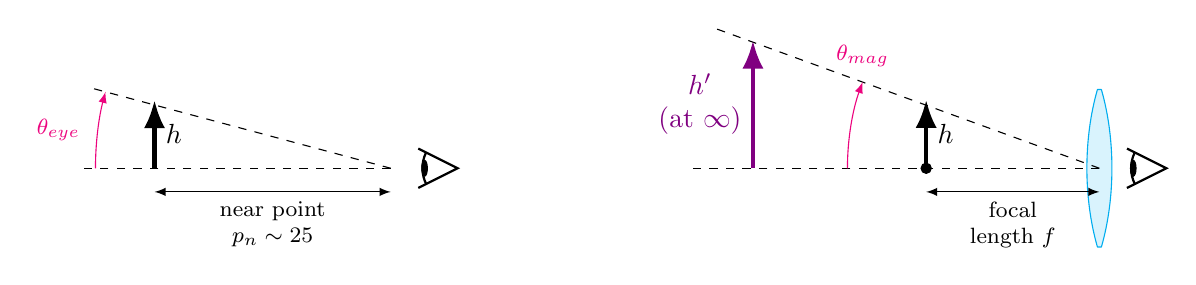
\begin{tikzpicture}
    % Draw the naked eye
    \begin{scope}
        \def\np{3}          % near point
        \def\offset{0.35}   % offset from the eye
        \def\viewAngA{15}   % viewing angle (left diagram)
        % Draw observer eyeball
        \draw[thick] (0,0.25) -- (0.5,0) -- (0,-0.25);
        \draw[thick] (0.1,-0.2) arc ({180+26.56}:155:0.45);
        \draw[fill=black] (0.08,0) ellipse (0.35mm and 1mm);
        % Draw naked eye max angle
        \draw[dashed] (-\offset, 0) -- (-\offset-1.3*\np, 0);
        \draw[dashed, rotate around={{360-\viewAngA}:(-\offset, 0)}] (-\offset, 0) -- (-\offset-1.3*\np, 0);
        \draw[-latex, RubineRed] (-1.25*\np-\offset, 0) arc[start angle=180, end angle={180-\viewAngA}, radius=1.25*\np] node[left=3, pos=0.5] {\footnotesize $\theta_\text{eye}$};
        % Draw the object at the near point
        \draw[ultra thick, -Latex] (-\np-\offset, 0) -- node[midway, right] {$h$} (-\offset-\np, {(\np+\offset)*sin(\viewAngA)});
        \draw[latex-latex] (-\np-\offset, -0.3) -- (-\offset, -0.3) node[pos=0.5, below, align=center] {\footnotesize near point\\[-0.25em]\footnotesize $p_n\sim\qty{25}{\centi\meter}$};
    \end{scope}
    %
    % Draw the eye with a magnifying lens
    \begin{scope}[shift={(9,0)}]
        \def\L{4}          % near point
        \def\f{2.2}         % focal length
        \def\offset{0.35}   % offset from the eye
        \def\viewAngB{20}   % viewing angle (left diagram)
        % Draw observer eyeball
        \draw[thick] (0,0.25) -- (0.5,0) -- (0,-0.25);
        \draw[thick] (0.1,-0.2) arc ({180+26.56}:155:0.45);
        \draw[fill=black] (0.08,0) ellipse (0.35mm and 1mm);
        % Draw a converging lens at the offset
        \draw[cyan, line join=round,fill=cyan!15] (-\offset+0.025,-1) coordinate (L1) arc (-30:30:1 and 2) coordinate (L2) -- ++(-0.05,0) arc (150:210:1 and 2) -- cycle;
        
        % \draw[cyan, line join=round,fill=cyan!15] (-\offset,-1) arc (-30:30:1 and 2) arc (150:210:1 and 2);
        % Draw naked eye max angle
        \draw[dashed] (-\offset, 0) -- (-\offset-1.3*\L, 0);
        \draw[dashed, rotate around={{360-\viewAngB}:(-\offset, 0)}] (-\offset, 0) -- (-\offset-1.3*\L, 0);
        \draw[-latex, RubineRed] (-0.8*\L-\offset, 0) arc[start angle=180, end angle={180-\viewAngB}, radius=0.8*\L] node[above=2] {\footnotesize $\theta_\text{mag}$};
        % Draw the object at the focal length
        \filldraw[black] (-\f-\offset, 0) circle (0.065);
        \draw[ultra thick, -Latex] (-\f-\offset, 0) -- node[midway, right] {$h$} (-\f-\offset, {(\f+\offset)*sin(\viewAngB)});
        \draw[latex-latex] (-\f-\offset, -0.3) -- (-\offset, -0.3) node[pos=0.5, below, align=center] {\footnotesize focal\\[-0.25em]\footnotesize length $f$};
        % Draw the image
        \draw[violet, ultra thick, -Latex] (-1.1*\L-\offset, 0) -- (-1.1*\L-\offset, {(1.1*\L+\offset)*sin(\viewAngB)}) node[pos=0.5, left, align=center] {$h'$\\(at $\infty$)};
    \end{scope}
\end{tikzpicture}
        \caption{Definition of the angles used in magnification power. Left: The naked eye observes an object at its near point subtending an angle $\theta_\text{eye}$. Right: when a convex lens is placed in front of the eye, and the object is located at the focal point of the lens such that $f$ is smaller than the near point $p_n$, the image subtends a larger angle $\theta_\text{mag}$, leading to a magnified virtual image.}
        \label{fig: magnification power}
    \end{figure}

    Figure~\ref{fig: magnification power} shows the geometry of an object of height $h$ placed at the near point of the eye. Suppose that $h\ll p_n$; for example, you are looking at very small text on a page at a distance $p=p_n\approx\qty{25}{\centi\meter}$. The angle subtended by the height of the text $h$ at your eye is given by
    %
    \begin{equation}\label{eq: max eye angle}
        \theta_\text{eye} \approx \tan{(\theta_\text{eye})} = \frac{h}{p_n} \approx \frac{h}{\qty{25}{\centi\meter}}
    \end{equation}
    %
    Now, if you put a converging lens in front of your eye and move the object to the point $p=f$, where $f<p_n$ the lens will produce a virtual upright image that appears to be at $i=\infty$ -- you can check with eq.~\ref{eq: thin lens equation} -- and will be in focus at your eye. We still have $h\ll f$, so the angle subtended by the object at distance $p=f$ is
    %
    \begin{equation}\label{eq: max mag angle}
        \theta_\text{mag} \approx \tan{(\theta_\text{mag})} = \frac{h}{f}.
    \end{equation}
    %
    The magnifying power of a simple lens, or its \textbf{angular magnification}, is defined by the ratio of $\theta_\text{mag}$, the apparent angular size of the object when it is at a distance $p=f$ from the lens, to $\theta_\text{eye}$, the apparent angular size of the object at your naked eye when the object is at your near point:
    %
    \begin{equation}\label{eq: angular magnification}
        m_\theta = \frac{\theta_\text{mag}}{\theta_\text{eye}} = \frac{h/f}{h/p_n} = \frac{p_n}{f} \approx \frac{\qty{25}{\centi\meter}}{f}.
    \end{equation}

    \subsection*{A Compound Microscope}

    To view very small objects, you can build a compound microscope using nothing more than two coaxial lenses separated by some distance. The lens closest to the object is called the \textbf{objective lens}, while the lens closest to your eye is called the \textbf{eyepiece}\footnote{Hopefully, the reasons for these names are obvious.}.

    \begin{figure}[ht]
        \centering
        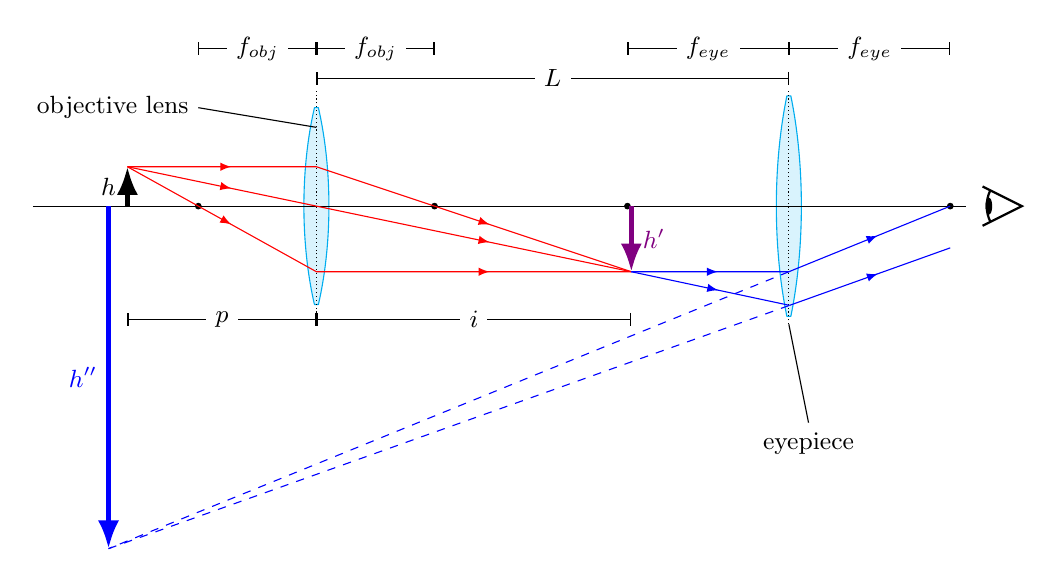
\begin{tikzpicture}

    \tikzset{
      % style to apply some styles to each segment of a path
      on each segment/.style={
        decorate,
        decoration={
          show path construction,
          moveto code={},
          lineto code={
            \path [#1]
            (\tikzinputsegmentfirst) -- (\tikzinputsegmentlast);
          },
          curveto code={
            \path [#1] (\tikzinputsegmentfirst)
            .. controls
            (\tikzinputsegmentsupporta) and (\tikzinputsegmentsupportb)
            ..
            (\tikzinputsegmentlast);
          },
          closepath code={
            \path [#1]
            (\tikzinputsegmentfirst) -- (\tikzinputsegmentlast);
          },
        },
      },
      % style to add an arrow in the middle of a path
      mid arrow/.style={postaction={decorate,decoration={
            markings,
            mark=at position 0.55 with {\arrow[#1]{latex}}
          }}},
    }

    \def\L{6}                       % microscope tube length
    \def\fobj{1.5}                  % objective focal length
    \def\feye{2.05}                 % eyepiece focal length
    \def\D{2.5}                     % objective diameter
    \def\De{2.8}                    % eyepiece diameter
    \def\h{0.5}                     % object height
    \def\p{1.6*\fobj}               % object-lens distance
    \def\i{{\fobj*\p/(\p-\fobj)}}   % image distance
    \def\m{{-\fobj/(\p - \fobj)}}   % magnification
    \def\hi{{-\fobj*\h/(\p-\fobj)}} % objective image height
    \def\ii{{-1.1*\p}}              % eyepiece image location
    \def\hii{-4.35}                 % eyepiece image height
    %
    % Compute angles
    \def\tanalpha{\h / (\p - \f)}
    \def\tanbeta{\h / (\p)}
%    \def\tangamma{{{\hi} / \feye}}
    %
    % Draw the objective lens
    \draw[cyan, line join=round,fill=cyan!15] (0.025,{-\D/2}) coordinate (L1) arc (-30:30:1 and \D) coordinate (L2) -- ++(-0.05,0) arc (150:210:1 and \D) -- cycle;
    \draw[densely dotted] (0,{-0.6*\D}) -- (0,{0.6*\D});
    \draw (0, {0.4*\D}) -- ++(-1.5,0.25) node[left] {\small objective lens};
    % Draw the eyepiece
    \draw[cyan, line join=round,fill=cyan!15] (\L+0.025,{-\De/2}) coordinate (L1) arc (-30:30:1 and \De) coordinate (L2) -- ++(-0.05,0) arc (150:210:1 and \De) -- cycle;
    \draw[densely dotted] (\L,{-0.6*\D}) -- (\L,{0.6*\D});
    \draw (\L, {-0.6*\D}) -- ++(0.25,-1.25) node[below] {\small eyepiece};
    %
    % Draw the axial line and focal points
    \draw ({-0.6*\L}, 0) -- ({\L+1.1*\feye}, 0);
    \filldraw[black] (-\fobj, 0) circle (0.035);
    \filldraw[black] (\fobj, 0) circle (0.035);
    \filldraw[black] ({\L-\feye}, 0) circle (0.035);
    \filldraw[black] ({\L+\feye}, 0) circle (0.035);
    %
    % Draw the object beyond the focal point
    \draw[ultra thick, -Latex] (-\p, 0) coordinate (O1) -- node[midway, left] {\small $h$} (-\p, \h) coordinate (O2);
%    %
%    % Draw rays from the object to the first real image through the objective
    \draw[red, postaction={on each segment={mid arrow=red}}] (O2) -- (0,\h) -- (\i, \hi);
    \draw[red, postaction={on each segment={mid arrow=red}}] (O2) -- (0,0) -- (\i, \hi);
    \draw[red, postaction={on each segment={mid arrow=red}}] (O2) -- (0, \hi) -- (\i, \hi);
    %
    % Draw the objective image
    \draw[ultra thick, violet, -Latex] (\i, 0) -- node[right] {\small $h'$} (\i, {\hi}) coordinate (O3);
    %
    % Draw rays from the first real image to the eyepiece and the final virtual image
    \draw[blue, postaction={on each segment={mid arrow=blue}}] (\i, \hi) -- (\L, \hi) -- ({\L+\feye}, 0);
    \draw[blue, dashed] ({\L}, \hi) -- (\ii, \hii);
    \draw[ultra thick, blue, -Latex] (\ii, 0) -- node[left, align=center]
    {\small $h''$} (\ii, \hii) coordinate (O4);
    \draw[blue, postaction={on each segment={mid arrow=blue}}] (O3) -- ++({0.98*\feye}, {-\feye*\tanbeta}) coordinate (O5);
    \draw[blue, dashed] (O4) -- (O5);
    \draw[blue, postaction={on each segment={mid arrow=blue}}] (O5) --
    ({\L+\feye}, -0.53);
    %
    % Draw the observer eyeball
    \begin{scope}[shift={(\L+1.2*\feye,0)}]
        \draw[thick] (0,0.25) -- (0.5,0) -- (0,-0.25);
        \draw[thick] (0.1,-0.2) arc ({180+26.56}:155:0.45);
        \draw[fill=black] (0.08,0) ellipse (0.35mm and 1mm);
    \end{scope}
    %
    % Label all lengths
    \draw[|-|] (-\fobj, {0.8*\D}) -- node[midway, fill=white] {\small $f_\text{obj}$} (0, {0.8*\D});
    \draw[|-|] (\fobj, {0.8*\D}) -- node[midway, fill=white] {\small $f_\text{obj}$} (0, {0.8*\D});
    \draw[|-|] ({\L-\feye}, {0.8*\D}) -- node[midway, fill=white] {\small $f_\text{eye}$} (\L, {0.8*\D});
    \draw[|-|] ({\L+\feye}, {0.8*\D}) -- node[midway, fill=white] {\small $f_\text{eye}$} (\L, {0.8*\D});
    \draw[|-|] (0, {0.65*\D}) -- node[midway, fill=white] {\small $L$} (\L, {0.65*\D});
    \draw[|-|] (-\p, {-0.575*\D}) -- node[midway, fill=white] {\small $p$} (0, {-0.575*\D});
    \draw[|-|] (0, {-0.575*\D}) -- node[midway, fill=white] {\small $i$} (\i, {-0.575*\D});
\end{tikzpicture}

        \caption{A basic compound microscope with an objective lens of focal length $f_\text{obj}$, an eyepiece of focal length $f_\text{eye}$, and a barrel length $L$ between the objective and eyepiece. Rays traced through the objective lens are drawn in red; rays traced through the eyepiece are drawn in blue.}
        \label{fig: compound microscope}
    \end{figure}

    The workings of the compound microscope are shown in Fig.~\ref{fig: compound microscope}. An object of height $h$ (black arrow) is positioned in front of an objective lens of focal length $f_\text{obj}$ such that $f_\text{obj}<p<2f_\text{obj}$. The \textbf{objective acts like a projector} and produces a magnified, inverted real image of size $h'$ near the focal length of the eyepiece (violet arrow). Following eq.~\ref{eq: thin lens magnification}, the objective provides a linear magnification
    \[
        m = -\frac{i}{p} = -\left(\frac{L-f_\text{eye}}{p}\right).
    \]
    
    The real image from the objective acts as the object for the eyepiece. With $h'$ located at $f_\text{eye}$, \textbf{the eyepiece acts like a simple magnifier} and produces a virtual image of height $h''$ (blue arrow) with rays that appear nearly parallel to the user. The angular magnification of the eyepiece, following eq.~\ref{eq: angular magnification}, is
    \[
        m_\theta = \frac{p_n}{f_\text{eye}} \approx \frac{\qty{25}{\centi\meter}}{f_\text{eye}}.
    \]
    The total magnification of the compound microscope is the product of the linear magnification of the objective and the angular magnification of the eyepiece:
    %
    \begin{equation}\label{eq: compound microscope}
        M = mm_\theta = -\left(\frac{L-f_\text{eye}}{p}\right)\left(\frac{\qty{25}{\centi\meter}}{f_\text{eye}}\right).
    \end{equation}

    \subsection*{An Astronomical Telescope}

    An astronomical telescope, shown in Figure~\ref{fig: astronomical telescope}, has a similar layout to the compound microscope, but instead of magnifying very nearby small features, it is designed to magnify very distant objects. It is designed such that $f_\text{obj}\gg f_\text{eye}$. For very distant objects ($p\to\infty$), we can treat rays from the object as if they are parallel. In this case, the objective focuses the rays at $i=f_\text{obj}$, as you would predict from the thin lens equation, producing a real inverted image of height $h'$. As in the compound microscope, the eyepiece acts like a simple magnifier, producing a virtual image of size $h''$ with rays nearly parallel at your eye. I.e., the virtual image is ``at infinity.''

    \begin{figure}[ht]
        \centering
        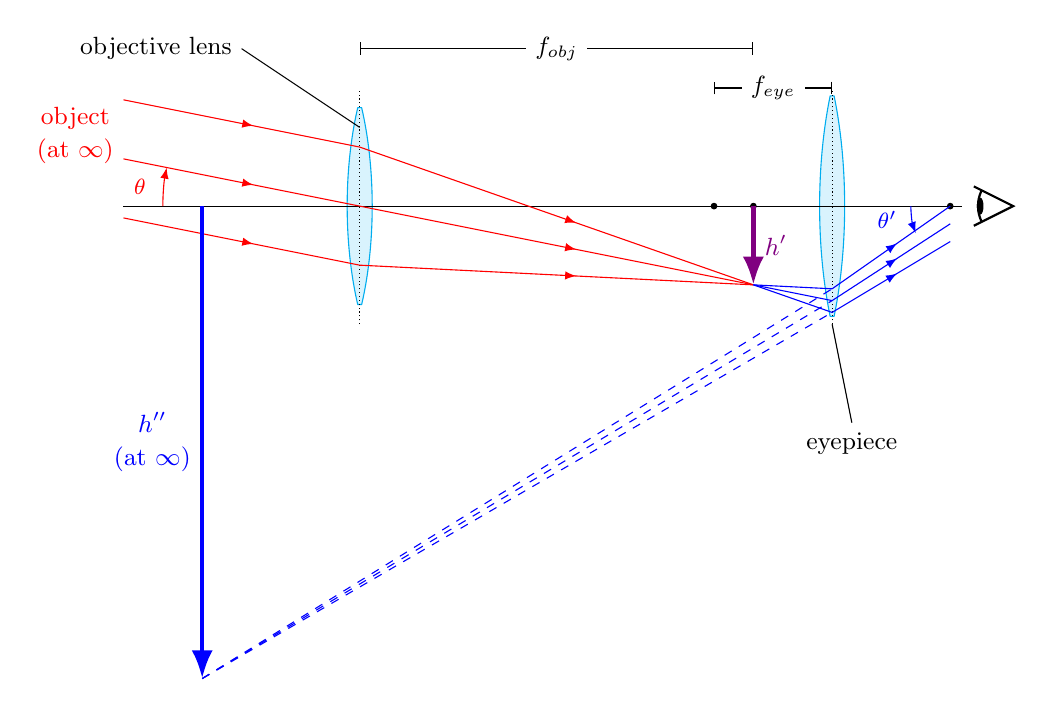
\begin{tikzpicture}

    \tikzset{
      % style to apply some styles to each segment of a path
      on each segment/.style={
        decorate,
        decoration={
          show path construction,
          moveto code={},
          lineto code={
            \path [#1]
            (\tikzinputsegmentfirst) -- (\tikzinputsegmentlast);
          },
          curveto code={
            \path [#1] (\tikzinputsegmentfirst)
            .. controls
            (\tikzinputsegmentsupporta) and (\tikzinputsegmentsupportb)
            ..
            (\tikzinputsegmentlast);
          },
          closepath code={
            \path [#1]
            (\tikzinputsegmentfirst) -- (\tikzinputsegmentlast);
          },
        },
      },
      % style to add an arrow in the middle of a path
      mid arrow/.style={postaction={decorate,decoration={
            markings,
            mark=at position 0.55 with {\arrow[#1]{latex}}
          }}},
    }

    \def\L{6}                       % microscope tube length
    \def\fobj{5}                    % objective focal length
    \def\feye{1.5}                  % eyepiece focal length
    \def\D{2.5}                     % objective diameter
    \def\De{2.8}                    % eyepiece diameter
    \def\h{0.5}                     % object height
    \def\hi{-1}                     % objective image height
    \def\i{{\fobj}}                 % objective image distance
    \def\offset{0.75}               % ray offsets for plotting
    \def\ii{-2}                     % eyepiece image location
    \def\hii{-6}                    % eyepiece image height
    %
    % Compute angles
    \def\thetaAng{11.3}
    \def\tantheta{-\hi / (\fobj)}
    \def\tanalpha{-(\offset + \hi)/(\fobj)}
    \def\tanbeta{(\offset - \hi)/(\fobj)}
    %
    % Draw the objective lens
    \draw[cyan, line join=round,fill=cyan!15] (0.025,{-\D/2}) coordinate (L1) arc (-30:30:1 and \D) coordinate (L2) -- ++(-0.05,0) arc (150:210:1 and \D) -- cycle;
    \draw[densely dotted] (0,{-0.6*\D}) -- (0,{0.6*\D});
    \draw (0, {0.4*\D}) -- ++(-1.5,1) node[left] {\small objective lens};
    % Draw the eyepiece
    \draw[cyan, line join=round,fill=cyan!15] (\L+0.025,{-\De/2}) coordinate (L1) arc (-30:30:1 and \De) coordinate (L2) -- ++(-0.05,0) arc (150:210:1 and \De) -- cycle;
    \draw[densely dotted] (\L,{-0.6*\D}) -- (\L,{0.6*\D});
    \draw (\L, {-0.6*\D}) -- ++(0.25,-1.25) node[below] {\small eyepiece};
    %
    % Draw the axial line and focal points
    \draw ({-0.5*\L}, 0) -- ({\L+1.1*\feye}, 0);
    \filldraw[black] (\fobj, 0) circle (0.035);
    \filldraw[black] ({\L-\feye}, 0) circle (0.035);
    \filldraw[black] ({\L+\feye}, 0) circle (0.035);
    %
    % Draw the objective image
    \draw[ultra thick, violet, -Latex] (\i, 0) -- node[right] {\small $h'$} (\i, {\hi}) coordinate (O3);
    %
    % Draw rays from infinity to the first real image through the objective
    \draw[red, postaction={on each segment={mid arrow=red}}] ({-0.5*\L}, {0.5*\L*\tantheta}) -- (0,0) -- (O3);
    \draw[red, postaction={on each segment={mid arrow=red}}] ({-0.5*\L}, {0.5*\L*\tantheta + \offset}) -- (0, \offset) -- (O3);
    \draw[red, postaction={on each segment={mid arrow=red}}] ({-0.5*\L}, {0.5*\L*\tantheta - \offset}) -- (0, -\offset) -- (O3);
    \draw[red] ({-0.5*\L}, {1.2*\offset}) node[left, align=center] {\small object\\ \small (at $\infty$)};
    \draw[-latex, red] (-2.5, 0) arc[start angle=180, end angle={180-\thetaAng}, radius=2.5] node[left=3, pos=0.5] {\footnotesize $\theta$};
    %
    % Draw rays from the first real image to the eyepiece and the final virtual image
    \draw[ultra thick, blue, -Latex] (\ii, 0) -- node[left, align=center] {\small $h''$\\ \small (at $\infty$)} (\ii, \hii) coordinate (O4);
    \draw[blue] (O3) -- ++({\L - \fobj}, {-(\L - \fobj)*\tanalpha}) coordinate (A);
    \draw[blue] (O3) -- ++({\L - \fobj}, {-(\L - \fobj)*\tantheta}) coordinate (B);
    \draw[blue] (O3) -- ++({\L - \fobj}, {-(\L - \fobj)*\tanbeta}) coordinate (C);
    \draw[blue, postaction={on each segment={mid arrow=blue}}] (A) -- ({\L+\feye}, 0);
    \draw[blue, postaction={on each segment={mid arrow=blue}}] (B) --
    ({\L+\feye}, -0.225);
    \draw[blue, postaction={on each segment={mid arrow=blue}}] (C) --
    ({\L+\feye}, -0.45);
    \draw[blue, dashed] (O4) -- (A);
    \draw[blue, dashed] (O4) -- (B);
    \draw[blue, dashed] (O4) -- (C);
    \draw[-latex, blue] ({\L+\feye-0.5}, 0) arc[start angle=180, end angle=200, radius=1] node[left=2, pos=0.5] {\footnotesize $\theta'$};
    %
    % Draw the observer eyeball
    \begin{scope}[shift={(\L+1.2*\feye,0)}]
        \draw[thick] (0,0.25) -- (0.5,0) -- (0,-0.25);
        \draw[thick] (0.1,-0.2) arc ({180+26.56}:155:0.45);
        \draw[fill=black] (0.08,0) ellipse (0.35mm and 1mm);
    \end{scope}
    %
    % Label all lengths
    \draw[|-|] (\fobj, {0.8*\D}) -- node[midway, fill=white] {\small $f_\text{obj}$} (0, {0.8*\D});
    \draw[|-|] ({\L-\feye}, {0.6*\D}) -- node[midway, fill=white] {\small $f_\text{eye}$} (\L, {0.6*\D});
\end{tikzpicture}
        \caption{A basic astronomical microscope with an objective lens of focal length $f_\text{obj}$ and an eyepiece of focal length $f_\text{eye}$. An object at $p=\infty$ sends parallel rays through the objective, which are focused at $i=f_\text{obj}$ (red arrows). The eyepiece produces a virtual image at $i'=\infty$ (blue arrows).}
        \label{fig: astronomical telescope}
    \end{figure}

    To estimate the magnification power of the telescope, we consider the angular magnification of the objective and the eyepiece. This differs from the compound microscope, where we considered the linear magnification of the objective lens. For an astronomical telescope, where the object of interest is effectively at $p=\infty$, and the object size could be gigantic\footnote{If we are looking at a planet or a star through the telescope, the object's size is much greater than the image size.}, it is much more sensible to use the apparent angular size.

    The apparent angular size of the real image from the objective is
    \[
        \theta \approx \tan{\theta} = \frac{h'}{f_\text{obj}},
    \]
    where we use a small-angle approximation. The apparent angular size of the virtual image from the eyepiece is
    \[
        \theta' \approx \tan{\theta'} = \frac{h'}{f_\text{eye}}
    \]
    The total magnification of the telescope is thus
    %
    \begin{equation}\label{eq: telescope magnification}
        M = \frac{\theta'}{\theta} 
        \approx \frac{\tan{\theta'}}{\tan{\theta}}
        = \frac{h'/f_\text{eye}}{h'/f_\text{obj}}
        = -\frac{f_\text{obj}}{f_\text{eye}},
    \end{equation}
    %
    where we inserted the minus sign to indicate that the telescope image is virtual.

    \subsection*{A Terrestrial Telescope (or Spyglass)}

    A terrestrial telescope, also known as a \textsl{spyglass} or an \textsl{opera glass}, is a two-lens system used for imaging distant objects. Like the astronomical telescope, it uses a long-focus objective lens and a short-focus eyepiece, but in the terrestrial telescope, a concave lens (also known as a ``meniscus'' lens) replaces the convex eyepiece. The magnification of a terrestrial telescope is given by eq.~\ref{eq: telescope magnification}.

    The first known terrestrial telescope, with $3\times$ magnification, was built by the Dutch lensmaker Hans Lippershey in 1608. Due to the concave lens at the eyepiece, the telescope produces an upright virtual image, making it useful for surveying and military applications. In 1609, Galileo Galilei refined Lippershey's design by replacing the concave eyepiece with a convex lens, allowing him to build astronomical telescopes with $30\times$ magnification. Using his device, Galileo rapidly published several revolutionary discoveries, including proof of the heliocentric model using the observed phases of Venus, mapping out the surface of the Moon, discovering the moons of Jupiter, observing Neptune, discovering Saturn's rings, and discovering that the Milky Way (which appears nebulous to the naked eye) is full of stars.

    % In this experiment, we use an optical bench: a magnetized track upon which various combinations of objects and lenses can be mounted. The \textsl{ object distance}, denoted $p$, is the distance between the object and the lens. Similarly, the distance from the lens to the image is the \textsl{image distance}, denoted $i$. Lastly, the \textsl{focal length} of a lens is denoted $f$. These three quantities are related by the \textsl{thin lens equation},
    % %
    % \begin{equation}\label{eq: thin lens equation}
    %     \frac{1}{f}=\frac{1}{p}+\frac{1}{i}
    % \end{equation}
    % %
    % You will construct four setups on the optical bench: a Projector, a Compound Microscope, and two long-range magnifiers: the Astronomical and Terrestrial Telescopes.
\end{theory}

\begin{experiment}

    \subsection*{Equipment}

    In this experiment, we use an optical bench: a magnetized track upon which various combinations of objects and lenses can be mounted. A picture of the track is shown in Figure~\ref{fig: thin lens setup}. The equipment needed for this lab is listed below:
    
    \begin{todolist}
        \item Box: Multiple lenses, holders, screen, object
        \item Light source
        \item 2 lengths of track
    \end{todolist}

    \begin{figure}[ht]
        \centering
        
\includegraphics[width=0.95\linewidth]{Lab 12: Geometric Optics/Projector1.png}
        \caption{Setup to test a projector lens and study the thin lens equation in eq.~\ref{eq: thin lens equation}.}
        \label{fig: thin lens setup}
    \end{figure}

    \subsection*{The Projector}
    
    In the first part of the experiment, you will build a \textbf{projector} using a single convex lens, an object to project, and a screen on which to view the projected image. A projector is a simple lens system that focuses an image onto a distant screen. By measuring pairs object and image distances, you will be able to experimentally determine the focal length of the convex lens using the thin lens equation in eq.~\ref{eq: thin lens equation}. Note that the thin-lens equation is an approximation; do not be disturbed if your results differ from those predicted by eq.~\ref{eq: thin lens equation}.

    \subsubsection*{Procedure}

    \begin{enumerate}
    
        \item Use the \qty{75}{\milli\meter} focal length convex lens (\#14), a crossed arrow target as the object (\#8), a viewing screen (\#11), and 2 element holders (\#22) to hold the lens and screen. Set up the optical bench as in Figure~\ref{fig: thin lens setup}. Place the lamp at one end of the bench and direct its illumination parallel to the bench axis using the knob on the top. You may attach the crossed arrow target directly to the lamp housing. Place the lens \qty{10}{\centi\meter} away from the crossed arrow target (i.e., set $p=\qty{10}{\centi\meter}$). Place the screen on the opposite side of the lens from the target. Adjust the screen to sharply focus the projected image.
        
        \item \label{step: thin lens obj dist} Measure the distance from the center of the lens to the plane of the screen, $i$, and the distance from the center of the lens to the object, $p$, and record these values in Data Table~\ref{data: projector} in the Postlab exercises. The image may seem to be in sharp focus over some measurable distance. Estimate this uncertainty in the image distance, $\Delta i$, and record it in Data Table~\ref{data: projector}.
        
        \item \label{step: thin lens description} Describe the image using the terms real or virtual, erect or inverted, magnified or reduced. It may be difficult to identify each pair definitively, but you should see a trend emerge.
        
        \item Repeat steps \ref{step: thin lens obj dist} and \ref{step: thin lens description} for many different object distances, exploring the range from \qty{10}{\centi\meter} to \qty{20}{\centi\meter} in increments of \qty{2}{\centi\meter}. Then complete the calculations in the Postlab exercises.
        
        % \item In \textbf{Section 4.1}, you will be asked to predict what value the image distance will approach as the object distance is increased. You may want to think about this now and test your hypothesis.
    
    \end{enumerate}

    \subsection*{The Magnifier}

    % The human eye can focus on objects located anywhere from infinity to a special point called the \textbf{near point}. The location of the near point varies from person to person, but its average value for the adult population is \qty{25}{\centi\meter} from the front of the eye.
    
    % If an object is placed closer than the near point, the rays from the object are too divergent for the eye to focus. However, by placing a converging lens between the object and the eye, the rays entering the eye become less divergent. In fact, if the object is placed at the focal point of the lens, the rays entering the eye appear to ``come from infinity.'' The eye has no problem focusing such rays on the retina.

    % When the focal length of the lens $f$ is less than the near point, and the object is placed at $f$, the image of the object appears magnified. The magnifying power of a lens, or its angular magnification, is defined by the ratio
    % %
    % \begin{equation}\label{eq: angular magnification}
    %     m = \frac{\theta_\text{mag}}{\theta_\text{eye}},
    % \end{equation}
    % %
    % where $\theta_\text{eye}$ is proportional to the maximum angular size of an object at the near point of your naked eye, and $\theta_\text{mag}$ is proportional to the maximum angular size of an image produced by a lens or system of lenses. These angles are best understood in reference to Figure~\ref{fig: magnification power}.

    % \begin{figure}[ht]
    %     \centering
    %     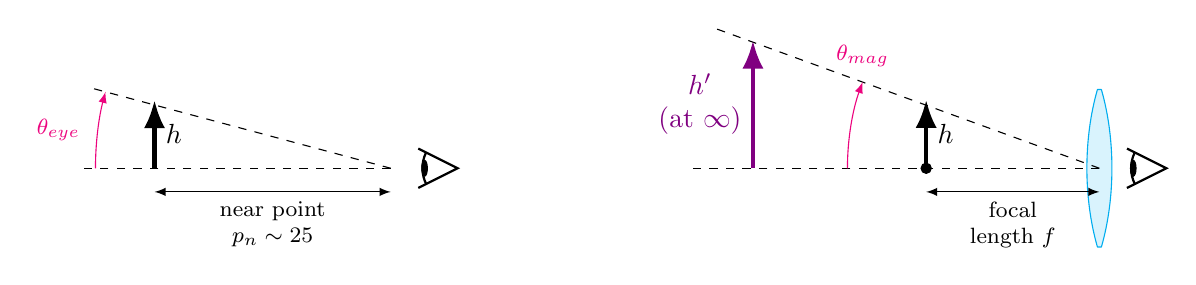
\begin{tikzpicture}
    % Draw the naked eye
    \begin{scope}
        \def\np{3}          % near point
        \def\offset{0.35}   % offset from the eye
        \def\viewAngA{15}   % viewing angle (left diagram)
        % Draw observer eyeball
        \draw[thick] (0,0.25) -- (0.5,0) -- (0,-0.25);
        \draw[thick] (0.1,-0.2) arc ({180+26.56}:155:0.45);
        \draw[fill=black] (0.08,0) ellipse (0.35mm and 1mm);
        % Draw naked eye max angle
        \draw[dashed] (-\offset, 0) -- (-\offset-1.3*\np, 0);
        \draw[dashed, rotate around={{360-\viewAngA}:(-\offset, 0)}] (-\offset, 0) -- (-\offset-1.3*\np, 0);
        \draw[-latex, RubineRed] (-1.25*\np-\offset, 0) arc[start angle=180, end angle={180-\viewAngA}, radius=1.25*\np] node[left=3, pos=0.5] {\footnotesize $\theta_\text{eye}$};
        % Draw the object at the near point
        \draw[ultra thick, -Latex] (-\np-\offset, 0) -- node[midway, right] {$h$} (-\offset-\np, {(\np+\offset)*sin(\viewAngA)});
        \draw[latex-latex] (-\np-\offset, -0.3) -- (-\offset, -0.3) node[pos=0.5, below, align=center] {\footnotesize near point\\[-0.25em]\footnotesize $p_n\sim\qty{25}{\centi\meter}$};
    \end{scope}
    %
    % Draw the eye with a magnifying lens
    \begin{scope}[shift={(9,0)}]
        \def\L{4}          % near point
        \def\f{2.2}         % focal length
        \def\offset{0.35}   % offset from the eye
        \def\viewAngB{20}   % viewing angle (left diagram)
        % Draw observer eyeball
        \draw[thick] (0,0.25) -- (0.5,0) -- (0,-0.25);
        \draw[thick] (0.1,-0.2) arc ({180+26.56}:155:0.45);
        \draw[fill=black] (0.08,0) ellipse (0.35mm and 1mm);
        % Draw a converging lens at the offset
        \draw[cyan, line join=round,fill=cyan!15] (-\offset+0.025,-1) coordinate (L1) arc (-30:30:1 and 2) coordinate (L2) -- ++(-0.05,0) arc (150:210:1 and 2) -- cycle;
        
        % \draw[cyan, line join=round,fill=cyan!15] (-\offset,-1) arc (-30:30:1 and 2) arc (150:210:1 and 2);
        % Draw naked eye max angle
        \draw[dashed] (-\offset, 0) -- (-\offset-1.3*\L, 0);
        \draw[dashed, rotate around={{360-\viewAngB}:(-\offset, 0)}] (-\offset, 0) -- (-\offset-1.3*\L, 0);
        \draw[-latex, RubineRed] (-0.8*\L-\offset, 0) arc[start angle=180, end angle={180-\viewAngB}, radius=0.8*\L] node[above=2] {\footnotesize $\theta_\text{mag}$};
        % Draw the object at the focal length
        \filldraw[black] (-\f-\offset, 0) circle (0.065);
        \draw[ultra thick, -Latex] (-\f-\offset, 0) -- node[midway, right] {$h$} (-\f-\offset, {(\f+\offset)*sin(\viewAngB)});
        \draw[latex-latex] (-\f-\offset, -0.3) -- (-\offset, -0.3) node[pos=0.5, below, align=center] {\footnotesize focal\\[-0.25em]\footnotesize length $f$};
        % Draw the image
        \draw[violet, ultra thick, -Latex] (-1.1*\L-\offset, 0) -- (-1.1*\L-\offset, {(1.1*\L+\offset)*sin(\viewAngB)}) node[pos=0.5, left, align=center] {$h'$\\(at $\infty$)};
    \end{scope}
\end{tikzpicture}
    %     \caption{Definition of the angles used in magnification power. Left: The naked eye observes an object at its near point subtending an angle $\theta_\text{eye}$. Right: when a convex lens is placed in front of the eye, and the object is located at the focal point of the lens such that $f$ is smaller than the near point $p_n$, the image subtends a larger angle $\theta_\text{mag}$, leading to a magnified virtual image.}
    %     \label{fig: magnification power}
    % \end{figure}

    % Suppose the height of the object is $h$. If we assume the angles are relatively small, then
    % %
    % \begin{align}
    %     \theta_\text{eye} &\approx \tan{(\theta_\text{eye})} = \frac{h}{p_n} = \frac{h}{\qty{25}{\centi\meter}}
    %     \label{eq: max eye angle}
    %     \\
    %     \theta_\text{mag} &\approx \tan{(\theta_\text{mag})} = \frac{h}{f}.
    %     \label{eq: max mag angle}
    % \end{align}
    % %
    % Thus, the magnification of the simple lens is
    % %
    % \begin{equation}\label{eq: simple lens magnification}
    %     m = \frac{\theta_\text{mag}}{\theta_\text{eye}} = \frac{\qty{25}{\centi\meter}}{f}.
    % \end{equation}
    % %
    % after combining eq.~\ref{eq: max eye angle} and \ref{eq: max mag angle}.

    \begin{figure}[h]
        \centering
        
\includegraphics[width=0.75\linewidth]{Lab 12: Geometric Optics/Magnifier.png}
        \caption{The setup for testing the magnification of a converging lens.}
        \label{fig: magnifier}
    \end{figure}
    \end{experiment}

    \subsubsection*{Procedure}

    \begin{enumerate}
        \item Estimate the location of your eye’s near point by holding the crossed arrow target at arm's length and slowly bringing it towards your eye, with one eye closed. Keep your eye relaxed and do not try too hard to keep the target in focus. As the target moves closer to your eye, there will be a point at which you can no longer focus easily on it. This is your eye's near point. Measure this distance from eye to target, taking care not to poke your eye out!
        
        \item Place a convex lens between your eye and the target (still at the near point). Verify that you can now focus on the target. The convex lens has allowed you to bring the object closer to your eye, thus making it appear larger. This is how a simple magnifier works. For the rest of this experiment, whenever an equation includes the population-average near point of $\overline{p}_n=\qty{25}{\centi\meter}$, substitute the measured value for your eye instead. \label{step: magnifier lens}

        \item Set up the magnifier as shown in Fig.~\ref{fig: magnifier}. Use the crossed arrow target as your object. Place the \qty{75}{\milli\meter} convex lens about \qty{2}{\centi\meter} away from the object and view it through the lens. Increase the object distance (the distance between the lens and the object) until the size of the image is maximized, yet still in focus. This should occur when the object distance is approximately equal to the focal length $f$. Note that beyond this point, the image becomes blurry. \label{step: magnifier distance}

        \item Measure the magnification of the lens using the following procedure. While looking through the lens at the object, hold a ruler between your eye and the lens and measure the apparent height of the object (the height of an arrow, for instance). Repeat the measurement again, holding your eye, the ruler, and the object in the same place, but with the lens removed from its holder. It may be helpful to have one person make the visual measurement while another person removes (and replaces) the lens. You may need to repeat this a few times to get the hang of it. Record your data, focal length, and image observations in Data Table~\ref{data: magnifier} in the Postlab exercises. \label{step: magnifier obs}

        \item Repeat steps \ref{step: magnifier lens} to \ref{step: magnifier obs} with a \qty{150}{\milli\meter} focal length convex lens.
    \end{enumerate}

    \subsection*{The Compound Microscope}

    The Compound Microscope (Figures~\ref{fig: compound microscope} and \ref{fig: compound microscope setup}) uses two lenses to create a magnified image of a very small, very close object.
    
    \begin{figure}[h]
        \centering
        
\includegraphics[width=0.75\linewidth]{Lab 12: Geometric Optics/Microscope.png}
        \caption{Setup for the compound microscope. Refer to Fig.~\ref{fig: compound microscope} and eq.~\ref{eq: compound microscope}.}
        \label{fig: compound microscope setup}
    \end{figure}

    \subsubsection*{Procedure}

    \begin{enumerate}
        \item Construct a compound microscope on the optical bench as in Figures~\ref{fig: compound microscope} and \ref{fig: compound microscope setup}. You may need to use 2 tracks to form one long bench. Use the \qty{75}{\milli\meter} convex lens as the objective and the \qty{150}{\milli\meter} convex lens as the eyepiece. Place the crossed arrow target \qty{12.5}{\centi\meter} in front of the objective lens. Start with the 2 lenses about \qty{50}{\centi\meter} apart. As you look through the microscope, move the eyepiece closer to the objective until you see a clearly focused image of the arrow target (perhaps only the center portion of the crossed arrow target).

        \item Measure the magnification of the system. Use the same method as was described in step~\ref{step: magnifier obs} of the procedure for the magnifier. This time, you will measure the apparent size of the arrows with both lenses in place, then with both lenses removed. Record your measured apparent heights in Data Table~\ref{data: microscope} in the Postlab exercises.
        
        \item While looking through the microscope, move the objective lens closer to the target and adjust the eyepiece as needed to keep the object in focus as well as you can.
        
        \item Record your data, the focal lengths, and your observations of the image in Data Table~\ref{data: microscope}.
    \end{enumerate}

    \subsection*{The Astronomical Telescope}

    The setup for an astronomical telescope is very similar to the compound microscope, except that you will remove the crosshair plate from the optical bench and look at objects at much greater distances.

    \subsubsection*{Procedure}

    \begin{enumerate}
        \item Construct an astronomical telescope on the optical bench as in Figure~\ref{fig: astronomical telescope}. Use the \qty{75}{\milli\meter} convex lens as your eyepiece and the \qty{150}{\milli\meter} lens as the objective lens. The distance between the two lenses will be approximately \qty{225}{\milli\meter}, the sum of the two focal lengths. Look at some reasonably distant object, perhaps a poster on the farthest wall in the lab room. Adjust the distance between the lenses to bring the object into sharp focus.

        \item Measure the magnification of the telescope. Use the same procedure for estimating magnification as was used in the previous two sections. Remember, measure the apparent height of the distant object with the two lenses in place and then with both lenses removed.
        
        \item Record your measurements, the focal lengths of both lenses, and observations of the image (inverted or upright, real or virtual, etc.) in Data Table~\ref{data: astronomical telescope} in the Postlab exercises.
    \end{enumerate}

    \subsection*{The Terrestrial Telescope}

    \subsubsection*{Procedure}

    \begin{enumerate}
        \item Construct a terrestrial telescope on the optical bench using the same lens for the objective as you did for the astronomical telescope (\qty{150}{\milli\meter} convex lens), but replace the convex eyepiece with a \qty{49}{\milli\meter} concave eyepiece (\#19). The focal length of the concave lens is $f_\text{eye}=-\qty{49}{\milli\meter}$.
        
        \item Put the eyepiece at one end of the optical bench. Place the objective about \qty{20}{\centi\meter} from the concave eyepiece and aim the telescope at a distant object, perhaps the same one used for the astronomical telescope in the previous section. Slowly move the objective toward the eyepiece until the distant object comes into focus.
        
        \item Measure the apparent magnification of the telescope using the same procedure as before. Measure the apparent height of the distant object with and without both lenses.
        
        \item Record your measurements, the focal lengths of both lenses, and observations of the image (inverted or upright, real or virtual, etc.) in Data Table~\ref{data: terrestrial telescope} in the Postlab exercises. 
    \end{enumerate}
    
\end{labsection}

\begin{postlab}

    %%% The Projector
    \fullwidth{\subsection*{The Projector (\pointsinrange{projector} points)}}

    \begingradingrange{projector}

        \filbreak
        \question[1] Add measurements from your study of the projector to Data Table~\ref{data: projector} and compute all derived quantities. To estimate the uncertainty on $1/i$, use propagation of uncertainties:
        \[
            \Delta(1/i) = \frac{\Delta i}{i^2}.
        \]

        \begin{center}
            \renewcommand{\arraystretch}{1.5}
            \captionsetup{font=normalsize}
            \captionof{data table}{Data for the projector measurements.\label{data: projector}}
            \begin{tabular}{|>{\centering\arraybackslash}p{1.4cm}|>{\centering\arraybackslash}p{1.4cm}|>{\centering\arraybackslash}p{1.8cm}|>{\centering\arraybackslash}p{4.5cm}|>{\centering\arraybackslash}p{1.4cm}|>{\centering\arraybackslash}p{1.4cm}|>{\centering\arraybackslash}p{1.4cm}|}
                \hline
                \rowcolor{gray!20}
                Object distance $p$ [cm] & Image distance $i$ [cm] & Image distance uncertainty $\Delta i$ [cm] & $\quad$Magnified / Reduced$\quad$ $\qquad$Real / Virtual$\qquad$ $\qquad$Inverted / Upright$\qquad$ & $1/p$ [cm$^{-1}$] & $1/i$ [cm$^{-1}$] & $\Delta(1/i)$ [cm$^{-1}$] \\ \hline
                & & & & & & \\ \hline
                & & & & & & \\ \hline
                & & & & & & \\ \hline
                & & & & & & \\ \hline
                & & & & & & \\ \hline
                & & & & & & \\ \hline
                & & & & & & \\ \hline
            \end{tabular}
        \end{center}
        %
        \begin{solution}[1cm]   
        \end{solution}

        \filbreak
        \question[1] As the object distance $p$ gets larger, the image distance $i$ approaches some value. Estimate this value by increasing the object distance, and observe the image distance.
        %
        \begin{solution}[4cm]
            
        \end{solution}

        \filbreak
        \question[2] In Graph~\ref{graph: projector}, plot $1/i$ versus $1/p$. Draw the calculated uncertainties on $1/i$ as error bars. Include labels and units for the axes. Draw a best-fit straight line through your data points. Determine the slope and $y$-intercept of this line. Show your work below.

        \begin{center}
        \captionsetup{font=normalsize}
        \captionof{graph}{Plot of $1/i$ vs. $1/p$ for the projector lens. \label{graph: projector}}
        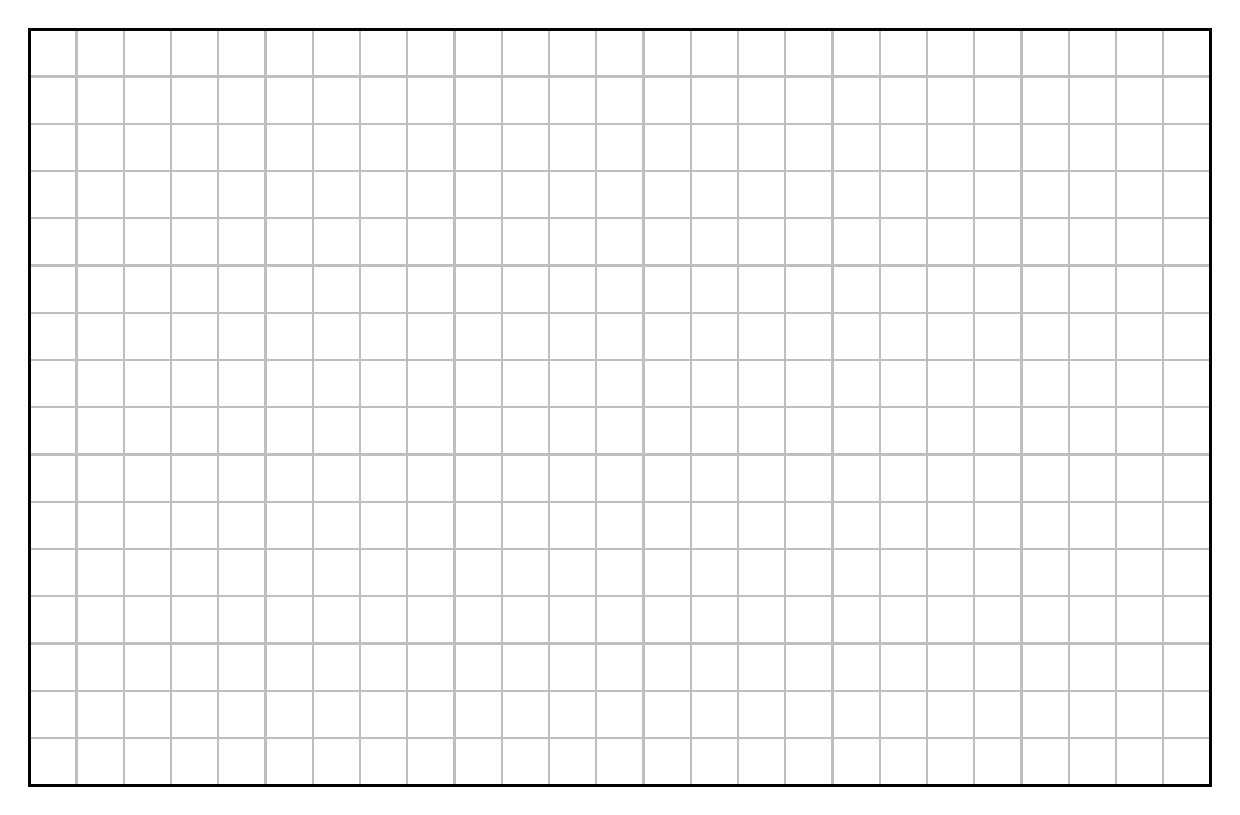
\begin{tikzpicture}
            % Define dimensions
            \def\gridwidth{25}
            \def\gridheight{16}
            \def\spacing{0.6}
            % Draw grid paper on the left
            \begin{scope}[xshift=0cm,yshift=0cm]
                % Major grid lines (thicker)
                \foreach \x in {0,1,...,\gridwidth}
                    \draw[gray!50,thick] (\x*\spacing,0) -- (\x*\spacing,\gridheight*\spacing);
                \foreach \y in {0,1,...,\gridheight}
                    \draw[gray!50, thick] (0,\y*\spacing) -- (\gridwidth*\spacing,\y*\spacing);
                \draw[black, very thick] (0,0) rectangle (\gridwidth*\spacing,\gridheight*\spacing);
            \end{scope}
        \end{tikzpicture}
        \end{center}
        %
        \begin{solution}[1cm]
        \end{solution}

        \filbreak
        \question[1] According to the plot in Graph~\ref{graph: projector}, what is the focal length of the lens used in the projector? Use the thin lens formula in eq.~\ref{eq: thin lens equation} and the equation for a line ($y=mx+b$).
        %
        \begin{solution}[2cm]
        \end{solution}

        \filbreak
        \question[1] Is the thin lens formula verified according to your data and Graph~\ref{graph: projector}? Explain your answer.
        %
        \begin{solution}[2cm]
        \end{solution}

    \endgradingrange{projector}

    %%% The Magnifier
    \pagebreak
    \fullwidth{\subsection*{The Magnifier (\pointsinrange{magnifier} points)}}

    \begingradingrange{magnifier}

        \filbreak
        \question[1] Add measurements from your study of the magnifier to Data Table~\ref{data: magnifier}.

        \begin{center}
            \renewcommand{\arraystretch}{2}
            \captionsetup{font=normalsize}
            \captionof{data table}{Data for the magnifier measurements.\label{data: magnifier}}
            \begin{tabular}{l>{\centering\arraybackslash}p{3cm}cl>{\centering\arraybackslash}p{3cm}}
                \hline
                & & & & \\
                \textbf{75~mm Lens} & & & \textbf{150~mm Lens} & \\
                height with lens: & & & height with lens: & \\
                \cline{2-2}\cline{5-5}
                height without lens: & & & height without lens: & \\
                \cline{2-2}\cline{5-5}
                $M_\text{75 mm}$ (measured): & & & $M_\text{150 mm}$ (measured): & \\
                \cline{2-2}\cline{5-5}
            \end{tabular}
        \end{center}
        %
        \begin{solution}[1cm]   
        \end{solution}

        \filbreak
        \question[1] Calculate the theoretical magnification of the \qty{75}{\milli\meter} lens and the \qty{150}{\milli\meter} lens using your near point. Show your work.
        %
        \begin{solution}[3cm]   
        \end{solution}

        \filbreak
        \question[2] How does your measured magnification compare to the theoretical magnification? Explain why it may or may not be so. Give specific reasons having to do with your measurement procedure.
        %
        \begin{solution}[3cm]   
        \end{solution}

    \endgradingrange{magnifier}

    %%% The Compound Microscope
    \pagebreak
    \fullwidth{\subsection*{The Compound Microscope (\pointsinrange{microscope} points)}}

    \begingradingrange{microscope}

        \filbreak
        \question[1] Add measurements from your study of the compound microscope to Data Table~\ref{data: microscope}.

        \begin{center}
            \renewcommand{\arraystretch}{2}
            \captionsetup{font=normalsize}
            \captionof{data table}{Data for the compound microscope.\label{data: microscope}}
            \begin{tabular}{l>{\centering\arraybackslash}p{3cm}cl>{\centering\arraybackslash}p{3cm}}
                \hline
                & & & & \\
                $f_\text{obj}$ [cm]: & & & height with lenses: & \\
                \cline{2-2}\cline{5-5}
                $f_\text{eye}$ [cm]: & & & height without lenses: & \\
                \cline{2-2}\cline{5-5}
                Barrel length $L$ [cm]: & & & $M$ (measured): & \\
                \cline{2-2}\cline{5-5}
            \end{tabular}
        \end{center}
        %
        \begin{solution}[1cm]   
        \end{solution}

        \filbreak
        \question[1] Calculate the theoretical magnification of your microscope using eq.~\ref{eq: compound microscope}. Show all work.
        %
        \begin{solution}[3cm]   
        \end{solution}

        \filbreak
        \question[1] Is your calculated magnification consistent with the measured value? Why or why not?
        %
        \begin{solution}[3cm]   
        \end{solution}

        \filbreak
        \question[1] Why does the magnification increase as the objective lens is moved closer to the object? What focusing problems tend to develop as the magnification increases?
        %
        \begin{solution}[3cm]   
        \end{solution}

    \endgradingrange{microscope}

    %%% The Astronomical Telescope
    \pagebreak
    \fullwidth{\subsection*{The Astronomical Telescope (\pointsinrange{astrotelescope} points)}}

    \begingradingrange{astrotelescope}

        \filbreak
        \question[1] Add measurements from your study of the astronomical telescope to Data Table~\ref{data: astronomical telescope}.

        \begin{center}
            \renewcommand{\arraystretch}{2}
            \captionsetup{font=normalsize}
            \captionof{data table}{Data for the astronomical telescope.\label{data: astronomical telescope}}
            \begin{tabular}{l>{\centering\arraybackslash}p{3cm}cl>{\centering\arraybackslash}p{3cm}}
                \hline
                & & & & \\
                $f_\text{obj}$ [cm]: & & & height with lenses: & \\
                \cline{2-2}\cline{5-5}
                $f_\text{eye}$ [cm]: & & & height without lenses: & \\
                \cline{2-2}\cline{5-5}
                Upright or inverted? & & & $M$ (measured): & \\
                \cline{2-2}\cline{5-5}
            \end{tabular}
        \end{center}
        %
        \begin{solution}[1cm]   
        \end{solution}

        \filbreak
        \question[1] Calculate the theoretical magnification of your astronomical telescope in eq.~\ref{eq: telescope magnification}. Show your work.
        %
        \begin{solution}[3cm]   
        \end{solution}

        \filbreak
        \question[1] Compare your calculated magnification to the measured one. Compute the percentage difference using the expression
        \[
            \left|\frac{M_\text{meas} - M_\text{calc}}{M_\text{calc}}\right|\times 100~[\%].
        \]
        Is it under 20\%? If not, explain why? Are they consistent? Why or why not?
        %
        \begin{solution}[3cm]   
        \end{solution}
    
    \endgradingrange{astrotelescope}

    %%% The Astronomical Telescope
    \pagebreak
    \fullwidth{\subsection*{The Terrestrial Telescope (\pointsinrange{terrtelescope} points)}}

    \begingradingrange{terrtelescope}

        \filbreak
        \question[1] Add measurements from your study of the terrestrial telescope to Data Table~\ref{data: terrestrial telescope}.

        \begin{center}
            \renewcommand{\arraystretch}{2}
            \captionsetup{font=normalsize}
            \captionof{data table}{Data for the terrestrial telescope.\label{data: terrestrial telescope}}
            \begin{tabular}{l>{\centering\arraybackslash}p{3cm}cl>{\centering\arraybackslash}p{3cm}}
                \hline
                & & & & \\
                $f_\text{obj}$ [cm]: & & & height with lenses: & \\
                \cline{2-2}\cline{5-5}
                $f_\text{eye}$ [cm]: & & & height without lenses: & \\
                \cline{2-2}\cline{5-5}
                Upright or inverted? & & & $M$ (measured): & \\
                \cline{2-2}\cline{5-5}
            \end{tabular}
        \end{center}
        %
        \begin{solution}[1cm]   
        \end{solution}

        \filbreak
        \question[1] Calculate the theoretical magnification of your terrestrial telescope in eq.~\ref{eq: telescope magnification}. Show your work.
        %
        \begin{solution}[3cm]   
        \end{solution}

        \filbreak
        \question[1] What is the main difference between the two telescopes' performance (other than the eyepiece)? When would you use the astronomical telescope? When would you use the terrestrial telescope?
        %
        \begin{solution}[3cm]   
        \end{solution}
    
    \endgradingrange{terrtelescope}
    
\end{postlab}

\end{document}